\chapter{Testing Framework}
Im folgenden Kapitel wird auf die einzelnen Komponenten des Test Frameworks eingegangen und deren Funktionsweise erläutert. Die Aufgabe des Test Frameworks liegt darin, die verschiedenen Prototypen, welche im Laufe dieser Semesterarbeit entwickelt wurden, mit diesem Framework einheitlich testen zu lassen. Das Test Framework wurde parallel zum RMIOnly- Systems mit Concurrency Control entwickelt.

\section{Konzept}
Das Framework lässt sich über eine Konfigurationsdatei konfigurieren und kann Testfälle, welche in einer XML Datenstruktur vorliegen, intepretieren und daraus die einzelnen Testszenarien generieren. Die Testszenarien werden vom Server auf die verfügbaren Testframework Clients verteilt und dort gestartet. Das Framework startet das zu testende System auf den verschiedenen Rechnern. Das zu testende System führt unmittelbar danach die Aktionen durch, welche im übergebenen Szenario definiert wurden.\newline
Die mit den Messwerten ausgefüllten Szenarien werden an den Server zurück\-geschickt und dort ausgewertet. Dies ermöglicht einen Vergleich der verschiedenen eingesetzten Algorithmen. Folgende Eckpunkte muss das Framework erfüllen:

\begin{itemize}
\item Die enwickelten Sys\-te\-me müssen sich ohne Programmcode- Anpassungen an das Framework anbinden lassen.
\item Das Framework muss die genauen Zeiten, welche für die Ausführungen der Operationen nötig waren, messen können.
\item Nach einem Testlauf muss ein Bericht erstellt werden können, welcher die nötigen Informationen darstellt.
\end{itemize}

\section{Allgemeine Informationen}
\label{sec:allgInformationen}

Um möglichst genaue Messdaten zu erlangen, wird das ganze System nach einem Testlauf beendet. Eine Aneinanderreihung von verschiedenen Test\-läufen würde die Messdaten aufgrund der JavaVirtualMachine be\-ein\-träch\-ti\-gen. Es besteht die Möglichkeit, dass für einen zweiten Testlauf weniger Speicher zur Verfügung steht, weil der Speicher immer noch mit Objekten des ersten Testlaufs besetzt ist. Da dies nicht mit Sicherheit überprüft werden kann, daher es kann nicht gewährleistet werden, dass die Grundvoraussetzungen für beide Testläufe gleich sind, wurde auf eine Aneinanderreihung von Testläufen verzichtet.

\section{Der Frameworkserver}
\label{sec:test-FW Server}
\subsection{Das Startup-Script}
\label{sec:startupScript}
Das  Startup-Script ist ein Shell-Script in der Bash-Sprache geschrieben. Das Script führt mehrere Methoden nacheinander aus:
\begin{enumerate}
\item Ein ant- Script wird an\-ge\-stos\-sen, wel\-ches die Pro\-jek\-te kom\-pi\-liert. Durch die\-sen Schritt ent\-stehen die .jar- Dateien, welche im nächs\-ten Schritt benötigt werden.
\item Das Script prüft die in der Config-Datei eingetragenen Zielrechner auf bereits vorhandene "client.jar"-Dateien und löscht diese Dateien, falls vorhanden.
\item Durch die Applikation "'Secure Copy" wird die zuvor im Buildprozess erstellte Datei "'client.jar" auf die Zielrechner kopiert.
\item Via SSH wird der Frameworkclient auf den Zielrechnern gestartet.
\item Der Frameworkserver wird gestartet.
\end{enumerate}
Sind diese Schritte abgeschlossen, beendet das Startupscript und die weitere Ausführung des Testlaufs wird durch den Frameworkserver orchestriert.
Beim Starten des Scripts wird der Name der Datei mitgegeben, in welcher der genaue Testlauf definiert ist. Wird kein Argument mitgegeben, läuft der Standardtestlauf ab, welcher in der Datei "'testCases.xml" beschrieben ist.\newline
Probleme beim Schreiben des Scripts waren selten. Ein Problem, welches gelöst werden musste, war der Umstand, dass das Script nach dem Starten eines Clients nicht mehr weiterlief, sondern einfach wartete. Dies war bei folgende Zeile der Fall:
\begin{lstlisting}[breaklines=true]
 ssh student@${i} "java -jar ${remotePath}/${clientJar}"
\end{lstlisting}	
Offensichtlich wartet das Script beim Ausführen eines Befehls auf einem fremden Rechner auf einen Rückgabewert in irgendeiner Form; also auf einen Errorcode oder aber auf einen Exitstatus. Das Absetzen dieses Befehls musste in einem seperaten Kind-Prozess stattfinden, damit der Eltern-Prozess die weiteren Aufgaben des Scripts abarbeiten konnte und nicht auf einen Rückgabewert wartete. Dies kann in der Bash-Shell mit einem "\&" erreicht werden. Die simple Lösung des Problems sieht schlussendlich fast gleich aus:
\begin{lstlisting}[breaklines=true]
 ssh student@${i} "java -jar ${remotePath}/${clientJar}" &
\end{lstlisting}

\subsection{Startprozess des Frameworkservers}
\label{sec:startFramework}
In diesem Kapitel werden die Schritte beschrieben, welche vor dem Starten des Testlaufs durchgeführt werden. Der Frameworkserver, einmal gestartet, administriert den ganzen weiteren Ablauf des Testlaufs. \newline
Die Kommunikation des Frameworkservers mit den Frameworkclients ist in folgendem Sequenzdiagramm grob dargestellt:


\begin{figure}[H]
\begin{center}
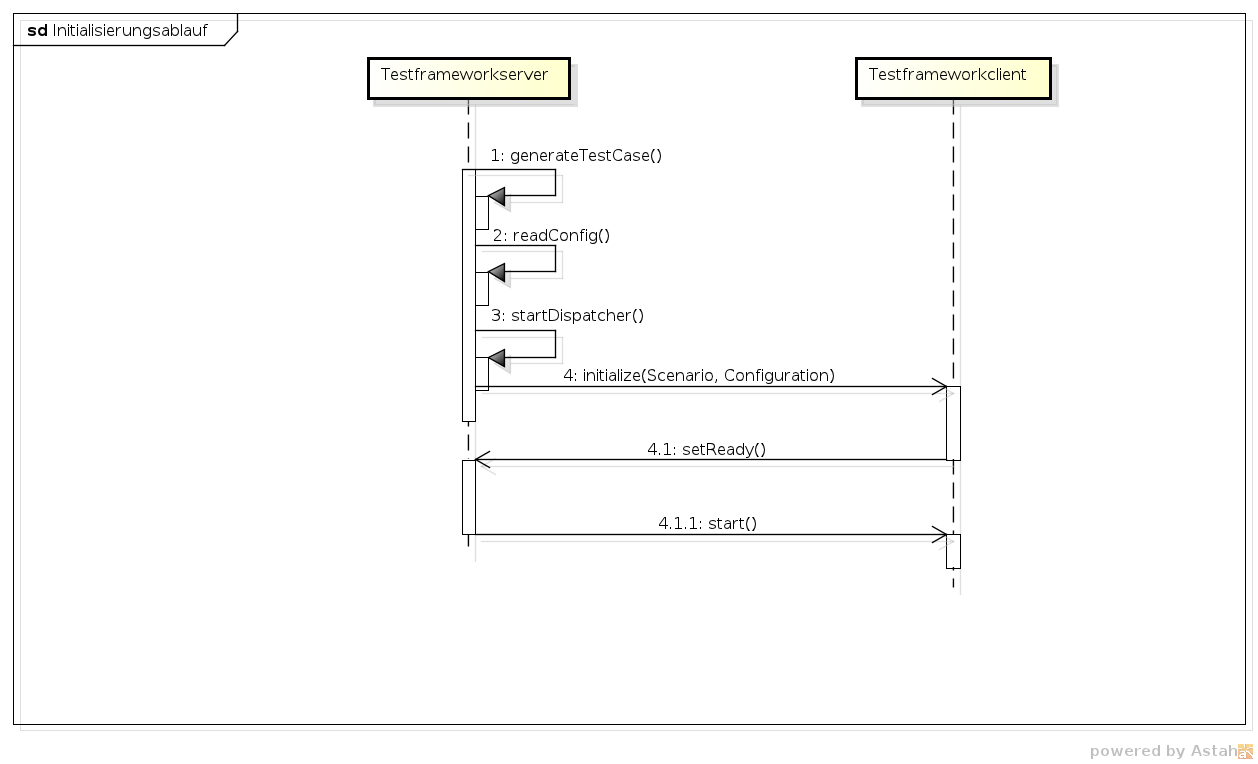
\includegraphics[scale=0.6]{image_testFramework/TestFWInit.png}
\end{center}
\caption{Testframework Init}
\end{figure}

Die im Diagramm dargestellten Operationen lassen sich wie folgt erklären:

\begin{itemize}
\item Die Methode \texttt{generateTestCase()} ruft eine Factory auf, welche aus einer XML-Datei einen Testcase generiert. Diese Factory wird unter dem Ka\-pi\-tel \ref{sec:testCaseFactory} "'Testcase-Factory" genauer be\-schrie\-ben.
\item Alle Konfigurationsparameter welche der Server braucht, sind in einer Konfigurations\-datei ab\-ge\-legt. Durch eine Configurationfactory wird durch mit Hilfe der Konfig\-urationsdatei ein Configuration- Objekt er\-zeugt. Unter dem Kapi\-tel \ref{sec:configurationFactory} "'Configuration Factory" wird dies näher beschrieben.
\item Nachdem die Konfigurationsparameter ausgelesen wurden, kann der Dis\-patcher in einem seper\-aten Thread ge\-startet werden. Weitere Aus\-füh\-run\-gen sind unter dem Kapitel \ref{sec:dispatcher} "'Der Dispatcher" zu finden.
\item Bei der Initialisierung der Clients, wird diesen je ein Szenario und ein Configuration-Objekt gesendet. Das Configuration-Objekt umfasst alle für den Client wichtigen Konfigurationsparameter, wie etwa die Ports, unter welchen der Server seine Dienste zur Verfügung stellt. Was ein Szenario genau ist, wird unter dem Kapitel \ref{sec:testCaseFactory} "'Testcase-Factory" genauer beschrieben.
\item Pro Client hat der Server beim Auslesen der Konfigurationsdatei ein Client-Objekt instanziert. Dies wurde voral\-lem zur Kon\-trol\-le der Cli\-ents durch den Server so implementiert. Darauf wird im Kapitel \ref{sec:clientObjekt} "'ClientObjekt" eingegangen.
\item Nachdem alle Clients \texttt{setReady()} aufgerufen haben, ruft der Server \texttt{start()} auf allen Clients auf. Dieser Vorgang wird unter dem Kapitel \ref{sec:startMethode} "'Start-Methode" genauer erläutert.
\end{itemize}

\subsubsection{Testcase-Factory}
\label{sec:testCaseFactory}
Die Testcase-Factory liest ein XML-File, in welchem ein sogenannter "TestCase" definiert ist. Wird beim Starten des Frameworkservers kein Paramter mitgegeben, wird der Standard-Testcase gewählt, welcher in der Datei "'testCases.xml" abgelegt ist. Wird aber ein Parameter mitgegeben, beschreibt dieser den Namen der auszuführenden TestCase-Datei.\newline
Durch die ein\-ge\-lesenen In\-for\-ma\-tio\-nen er\-stellt die Fac\-tory die Szena\-rien, wel\-che dann wei\-ter an die ver\-schie\-denen Clients ge\-sendet werden. Folgender Block ist ein Auszug aus einer TestCase-Datei:

\begin{lstlisting}[language=XML, breaklines=true] 	
<?xml version='1.0' encoding='UTF-8'?>
<TestRun>
  <TestCase SystemUnderTest="ch.hsr.objectCaching.rmiOnlyClient.RMIonlyClientSystem">
    <Account balance="1"></Account>
      <Scenario id="1">
        <ActionSequence>
          <Increment count ="100" delay="0" factor="1.1"></Increment>
	</ActionSequence>
      </Scenario>
      <Scenario id="2">
	<ActionSequence>
          <Increment count ="100" delay="0" factor="1.1"></Increment>
	</ActionSequence>
      </Scenario>
  </TestCase>
</TestRun>
\end{lstlisting}

Das Attribut "'SystemUnderTest" definiert das zu testende System. Der Vorteil dieser Methode ist, dass das zu testende System einfach in XML angegeben wird und dann getestet werden kann. Es müssen so keine Anpassungen am Code vorgenommen werden, egal welches System getestet werden soll. Somit spielt es für das Framework keine Rolle, welches System getestet werden soll.\newline
Eine TestCase-Datei beschreibt genau einen TestCase. Ein Test\-Case kann ver\-schie\-dene Sze\-na\-ri\-en be\-in\-hal\-ten, oder aber auch nur ein Szena\-rio be\-schrei\-ben. Ist nur ein Sz\-enario definiert, werden beide Clients mit dem\-selben Szenario arbeiten. Falls mehrere Szenarien beschrieben sind, werden die Clients unterschiedliche Szenarien durchführen. \newline
Aus obigem XML-Code generiert die Factory nun ein Objekt vom Typ TestCase. Dieses Objekt definiert nun zwei Szenarien, welche wiederum aus mehreren Actions bestehen. Was genau eine Action ist, ist unter dem Kapitel \ref{sec:action} "'Actions" beschrieben. Die Factory wird nun bei diesem Beispielcode eine Abfolge von 100 "'Increment-Action" erstellen und diese in das Scenario-Objekt ablegen.


\subsubsection{Configuration-Factory}
\label{sec:configurationFactory}
Die Configuration-Factory liest alle Daten aus der Konfigurationsdatei aus und erstellt mit diesen Informationen ein Configuration-Objekt. Die Konfigurationsdatei sieht wie folgt aus:
\begin{lstlisting}
Client0=152.96.193.18
Client1=152.96.193.19
Clientport=36927
ServerRmiPort=36925
ServerSocketPort=36926
ServerRegistryName=Server
ClientRegistryName=Client
\end{lstlisting}

In der Konfigurationsdatei ist definiert, welche Clients auf welchem Port kontaktiert werden können. Weiter ist der Registry-Name definiert, damit der Server weiss, über welche Registry er die Methoden auf dem Client aufrufen muss. \newline
Aus diesen Informationen erstellt die Factory ein Configuration- Objekt, welches sie dem Client als erstes sendet. Damit ist gewährleistet, dass der Frameworkserver und die Frameworkclients miteinander über RMI kommunizieren können. \newline
Pro Client, welcher in der Konfigurationsdatei definiert ist, wird ein Client-Objekt instanziert, was im folgenden Kapitel beschrieben wird.

\subsubsection{ClientObjekt}
\label{sec:clientObjekt}

Das Clientobjekt besitzt unter anderem ein Datenfeld, welches genau zwei Zustände annehmen kann: Ready und NotReady. Führt der Frameworkclient die Methode \texttt{setReady()} auf dem Server aus, wird der Status auf dem jeweiligen Objekt auf Ready gesetzt. Folgend die Implementation der setReady-Methode:
\begin{lstlisting}[language=Java, breaklines=true]
public void setReady(String ip) 
{
	logger.info("Setted ready with: " + ip);
	Client temp;
	if((temp = clientList.getClientByIp(ip)) != null)
	{
		temp.setStartingState(StartingState.READY);
	}
	if(checkAllReady())
	{
		start();
	}
}
\end{lstlisting}

Interessant an dieser Methode ist die Funktion der \texttt{checkAllReady}-Methode. Dieser Mecha\-nismus ist nicht nur dazu da, um alle Clients mög\-lichst gleichzeitig zu starten, sondern auch, um die Threads zu steuern. Die Methode \texttt{setReady()} wird durch mehrere verschiedene Threads aufgerufen, von jedem Client genau ein Mal. Durch die Implementation von \texttt{checkAllReady()} wird aber nur der letzte Thread, welcher \texttt{setReady()} aufruft, weiterleben und \texttt{start()} ausführen können. Somit ist garantiert, dass auch danach nur ein Thread aktiv ist und keine Seiteneffekte entstehen können.\newline
Die Implementation dieser Logik war nicht schwer, doch das Bewusstsein für die Problematik mit mehreren Threads muss ständig vorhanden sein. Die Einflüsse der parallelen Programmierung stellten ohnehin einen spannenden Aspekt dieser Arbeit dar. 

\subsubsection{Die Start-Methode}
\label{sec:startMethode}

Die Methode \texttt{start()} gibt dem Client an, mit der Abarbeitung des Szenarios zu beginnen. Die erste Implementation dieser Methode sah wie folgt aus:
\begin{lstlisting}[language=java, breaklines=true]
private void start()
{
	logger.info("Method start() invoked");
	for(int i = 0; i < clientList.size(); i++)
	{
		clientList.getClient(i).getClientStub().startTest();
	}
}
\end{lstlisting}

Nach einigen Testdurchläufen konnte festgestellt werden, dass die Clients ihre Szenarien nur sequentiell abarbeiteten und die Operationen auf dem Server nicht gleichzeitig geschehen. Schuld an diesem Umstand war obige Implementation der \texttt{start}-Methode. Der Server-Thread, welcher \texttt{startTest()} auf dem Client aufrief, wartete solange, bis die Methode zurückkehrte. Da die Methode natürlich erst nach der Beendigung des Szenarios zurückkehrt, konnte nur immer genau ein Client zu einem gewissen Zeitpunkt aktiv sein.\newline
Die jetzige Implementation und somit die Lösung des Problems sieht wie folgt aus:
\begin{lstlisting}[language=java, breaklines=true]
private void start()
{
	logger.info("Method start() invoked");
	for(int i = 0; i < clientList.size(); i++)
	{
		ClientStart clientStart = new ClientStart(clientList.getClient(i));
		new Thread(clientStart).start();
	}
}
\end{lstlisting}
Um das Problem mit der Erstellung eines neuen Threads für jeden zu startenden Client zu umgehen, musste eine weitere Klasse Namens "'ClientStart" ge\-schrie\-ben wer\-den. Die Klas\-se im\-p\-le\-men\-tiert natür\-lich das Inter\-face "'Run\-nable" und im\-p\-le\-men\-tiert die "'run()"'-Methode wie folgt:
\begin{lstlisting}[language=java, breaklines=true]
public void run() {
	try {
		client.getClientStub().startTest();
	} catch (RemoteException e) {
		logger.log(Level.SEVERE, "Uncaught exception", e);
	}
}
\end{lstlisting}

Mit dieser Implementation wird der Methodenaufruf "start()" nun von einem seperaten Thread ausgeführt. Dies führt dazu, dass die Clients nun zeitlich parallel gestartet werden und nicht nacheinander. Da die einzelnen Threads nach Beendigung der \texttt{run()}-Methode sterben, ist die Art der Implementation unbedenklich bezüglich Seiteneffekte oder "'Zombie-Threads".

\subsubsection{Der Dispatcher}
\label{sec:dispatcher}

Der Dispatcher stellt die Verbindung zwischen dem Frameworkserver und dem Server des Systems, welches getestet werden soll, dar. Dem Dispatcher wird die Portnummer angegeben, unter welcher er ein Socket öffnen soll. Weiter wird ihm ein String übergeben, in welchem der Pfad des zu testenden Systems drinnsteht. Der Dispatcher instanziert daraufhin das zu testende System mit Hilfe des Strings und wartet danach in einem blockierten Zustand auf sich verbindende Clients. Nachdem ein Client auf dem geöffneten Socket eine Verbindung aufgebaut hat, übergibt der Dispatcher die Verbindung in Form eines Input und eines Outputstreams dem Server des zu testenden Systems.\newline
Logischerweise läuft der Dispatcher wiederum in einem seperaten Thread.

\subsection{Herunterfahren des Frameworkservers}
\label{sec:herunterfahrenFramework}

Nach Beendigung eines Testlaufs, muss der Server mehrere Arbeiten erledigen. Nachfolgend werden die wichtigsten Aufgaben aufgeführt:


\begin{figure}[H]
\begin{center}
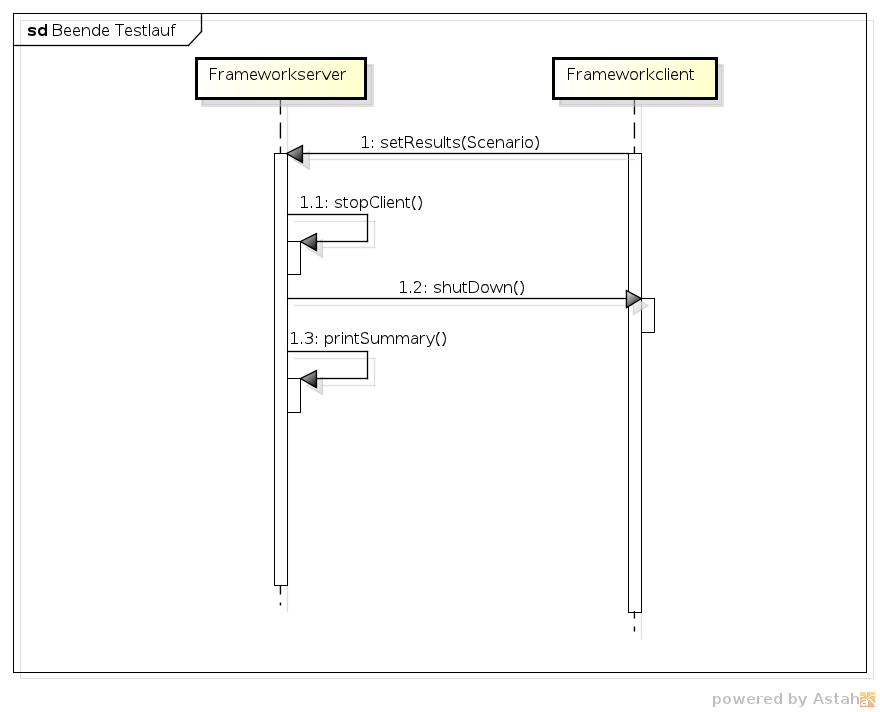
\includegraphics[scale=0.6]{image_testFramework/BeendeTestlauf.png}
\end{center}
\caption{Testfamework Exit}
\end{figure}

Die im Diagramm ersichtlichen Operationen können folgender\-massen er\-läu\-tert werden:
\begin{itemize}
\item Die Methode \texttt{setResults(Scenario)} wird vom Client auf dem Server auf\-ge\-rufen, durch den Aufruf dieser Methode weiss der Server, dass der aufrufende Client sein Szenario durchgespielt hat. Weiter wird mit dem Aufruf der Methode wiederum ein Thread durch den RMI-Daemon gestartet, welcher die weiter folgenden Methoden anstösst.
\item Aus der \texttt{setResults(Scenario)}- Methode wird di\-rekt "'stopClient()" auf\-ge\-rufen. Was diese Methode genau macht, wird im Kapitel \ref{sec:stopClient} "'Stoppen eines Clients" genau beschrieben.
\item Die Methode \texttt{shutDown()} wird auf dem Client aufgerufen. Der Client trennt daraufhin die RMI-Verbindung zum Server und schaltet sich selber ab. Nähere Informationen zum Abschaltungsprozess eines Clients kann unter dem Kapitel \ref{sec:test-FW Client} "'Testframework Client" nachgelesen werden.
\item Die Methode \texttt{printSummary()} verwertet die Ergebnisse, welche die Clients in ihrem Szenario gespeichert und wieder übertragen haben. Mehr Informationen dazu im Kapitel \ref{sec:reportGenerator} "'Report Generator". Weiter wird auf der Console ausgegeben, ob es "Lost-Update"-Probleme gegeben hat oder nicht. Mehr zu diesem Thema unter dem Kapitel \ref{sec:resultGenerator}"'Result Generator".
\end{itemize}

\subsubsection{Stoppen eines Clients}
\label{sec:stopClient}
Ruft ein Client die Methode \texttt{setResults(Scenario)} auf dem Server auf, wird Serverintern der Status des Clients auf "Down" gesetzt. Da die Methode \texttt{stopClient()} wiederum pro Client genau ein Mal aufgerufen wird, entsteht das Problem, dass mehrere Threads am Leben sind. Um dies ab einem gewissen Punkt zu verhindern, wurde ähnlich zur \texttt{setReady()}-Methode, folgende Implementation gewählt:
\begin{lstlisting}[language=java, breaklines=true]
private void stopClient(String clientIp)
{
	Client temp;
	try {
		
		if((temp = clientList.getClientByIp(clientIp)) != null)
		{
			logger.info("stop client with ip: " + clientIp);
			temp.setClientRunning(ShutedDown.DOWN);
			temp.getClientStub().shutdown();
		}
	} catch (RemoteException e) {
		logger.log(Level.SEVERE, "Uncaught exception", e);
	}
	if(checkAllShutedDown())
	{
		printSummary();
	}
}
\end{lstlisting}

Durch die Prüfung \texttt{checkAllShutedDown()}, wird nur der letzte aller Threads weiterleben. Somit wird auch nur ein Thread fähig sein die Methode \texttt{printSummary()} auszuführen, während die anderen Threads die Methode zu Ende abarbeiten und am Ende der Methode sterben. Durch diese Implementation wird sichergestellt, dass nur ein Thread weiterlebt und keine "'Zombi-Prozesse" mehr vorhanden sind.\newline
Weiter wird beim Abarbeiten dieser Methode die Methode \texttt{shutdown()} auf dem Client aufgerufen. Nach diesem Aufruf fährt sich der Client herunter und kappt alle akiven Verbindungen zum Server. Weitere Informationen zum Shutdown-Prozess des Clients sind unter der Kapitel des Frameworkclients ersichtlich.\newline
Oben genannte Implementation der \texttt{stopClient(String clientIP)}-Methode hat lange funktioniert. Während des Entwicklungsprozesses der RMI-Only Lösung lief das Framework mit der erwähnten Methode ohne Probleme. Bei den ersten Testläufen der RMI-Cache Lösung wurden beim Herunterfahren der Umgebung allerdings Exceptions generiert. Da die Fehlersuche bei Software mit einer Vielzahl von Threads sehr langwierig ist, nahm die Analyse des Fehlers viel Zeit in Anspruch.\newline 
Schlussendlich wurde bemerkt, dass die Methode \texttt{printSummary()} trotz aller Vorsichtsmassnahmen von jedem Client ein Mal ausgeführt wurde, was dazu führte, dass mehrere Zusammenfassungen generiert wurden und probiert wurde, den FrameworkServer mehrere Male herunterzufahren. Der Versuch den FrameworkServer mehrmals herunterzufahren war natürlich der Grund für die Ex\-cep\-tions, da dem zweiten Client ein\-fach der Ver\-bin\-dungs\-part\-ner weggerissen wurde.\newline
Der Grund des Fehlverhaltens lag in der nicht-funktionierenden Barriere \texttt{checkAllShutedDown()}. Nachdem der Methodenkopf durch "'synchronized" erweitert wurde, funktionierte das Framework wieder problemlos:
\begin{lstlisting}[language=java, breaklines=true]
synchronized private void stopClient(String clientIp)
\end{lstlisting}
Anscheinend sind die Clients bei der Cache- Implementation immer zum fast gleichen Zeit\-punkt fer\-tig, was dazu führte, dass der Sta\-tus "'ShutedDown.DOWN" nur un\-zu\-ver\-läs\-sig gesetzt wurde.\newline
Das Fehlerszenario lief wie folgt ab:
\begin{itemize}
\item Thread1 betritt die \texttt{stopClient(String clientIp)}-Methode und setzt seinen Status auf DOWN.
\item Kurz nachdem Thread1 seinen Status gesetzt hat, wird im die Res\-sour\-ce entzogen und Thread2 kommt zum Zug.
\item Thread2 betritt nun seinerseits die Methode und setzt seinen Status ebenfalls auf DOWN.
\item Da nun alle Threads auf DOWN sind, wird die Barriere nicht mehr funktionieren und mehrere Threads führen \texttt{printSummary()} aus.
\end{itemize}
Dadurch, dass die Methode nun synchronized ist, ist gewährleistet, dass sich nur ein Thread in der Methode aufhalten kann. Das wiederum bedeutet, dass die Barriere \texttt{checkAllShutedDown()} nun wie gewohnt funktioniert, da die Stati der Threads wieder zuverlässig gesetzt werden.

\subsubsection{Report Generator}
\label{sec:reportGenerator}

Beim Aufruf der Methode \texttt{printSummary()}, wird ein ReportGenerator instanziert, welche die Daten der Clients ausliest und in eine Textdatei schreibt. Folgende Werte wurden durch die Clients erfasst:
\begin{itemize}
\item Zeit, welche benötigt wurde um die entsprechende Action durch\-zu\-führen.
\item Protokollierung, ob bei der Durchführung ein Konflikt generiert wurde oder nicht.
\item Zeit, welche in einem Konfliktfall gebraucht wurde, um den Konflikt zu behandeln und die Operation noch einmal auszuführen.
\end{itemize}

Pro Client wird eine Datei erstellt, in welcher die Daten dargestellt werden. Folgend einen kurzen Auszug eines solchen Reports:

\begin{lstlisting}[breaklines=true]
**************************************************
Result for Client: 152.96.193.18 with ScenarioID: 1
OS: Linux / 3.0.0-17-generic-pae
**************************************************
ActionNr;#ofTries;Time[ms];ACTION
0;0;42.674487;INCREMENT(READ) WITHOUT DELAY
0;1;77.969046;INCREMENT(WRITE) WITHOUT DELAY
1;0;79.684003;INCREMENT(READ) WITHOUT DELAY
1;1;81.984427;INCREMENT(WRITE) WITHOUT DELAY

------------------------------------------------
100% of all Action executed are successful
Total actions executed: 2, number of unsuccessful action 0
Total getBalance calls: 2, avg. execution time 61.179245
Total setBalance calls: 2, avg. execution time 79.9767365

Total Conflict: 0 / Gesamt Dauer: 282.311963 ms / durch. Dauer pro Operation: 141.1559815
\end{lstlisting}

Die genaue Messerwerte, mit Durch\-schnitts\-wer\-ten und Ver\-gleiche zwischen den verschiedenen Systemen sind am Schluss dieser Arbeit zu finden. \newline
Während der Entwicklung des Frameworks und der verschiedenen Systeme, schien die Ausgabe der Testergebnisse in eine Textdatei eine gute Idee zu sein. Während den Messungen des Systems wurde aber bemerkt, dass dies eine äusserst zeitraubende und mühsame Arbeit nach sich zieht: Für einen Testcase mit acht Clients, bei welchem der Messgenauigkeit zu liebe drei Durchläufe getätigt werden, fallen insgesamt 24 Textdateien an. Um einen Mittelwert der Ergebnisse zu bekommen, müssen alle Textdateien geöffnet werden, die Mittelwerte müssen berechnet werden und in einer weiteren Datei abgelegt werden. \newline
Dieser Umstand wurde erst am Ende der Arbeit bemerkt, weshalb auf eine aufwändige Lösung verzichtet wurde. Mögliche Lösungsansätze für dieses Problem wären aber:
\begin{itemize}
\item Die Ergebnisse werden in eine Datenbank geschrieben.
\item Die Ausgabe erfolgt in ein XML-File.
\end{itemize}
Die Ausgabe der Ergebnisse in eine Datenbank wäre die sauberste Lösung, ist jedoch auch mit sehr viel Aufwand verbunden. Ein XML-File wäre sicher einfacher zu handhaben, als die Textdateien und hätte schlussendlich weniger Aufwand für die Messungen bedeutet.

\subsubsection{Result Generator}
\label{sec:resultGenerator}
Der ResultGenerator ist ein Generator, welcher für die Berechnung des zu erwartenden Endbestandes des Account-Objektes verantwortlich ist. Wenn alle Clients ihre Operationen abgeschlossen haben, wird das aktuelle Ergebnis des Account-Objektes und das erwartete Ergebnis auf der Konsole ausgegeben. Zusätzlich wird kontrolliert, ob die Ergebnisse übereinstimmen und eine entsprechende Meldung wird auf der Konsole ausgegeben:
\begin{lstlisting}[breaklines=true]
19.04.2012 18:33:38 ch.hsr.objectCaching.testFrameworkServer.Server printSummary
INFO: AccountBalance is: 1.4641001269340557
19.04.2012 18:33:38 ch.hsr.objectCaching.testFrameworkServer.Server printSummary
INFO: AccountBalance should be: 1.4641001269340557
19.04.2012 18:33:38 ch.hsr.objectCaching.testFrameworkServer.Server printSummary
INFO: No Lost-Updates!
\end{lstlisting}

\subsubsection{Logger}
\label{sec:logger}
Wie in dem Konsolenauszug unter "'Result Generator" gesehen werden kann, wurde ein Logger eingebaut, welcher alle Methodenaufrufe protokoliert. Der Logger schreibt die Ereignisse erstens auf die Konsole und zweitens schreibt er alle Informationen zu einem Methodenaufruf in eine Datei. Diese Logdatei ist sehr Informationsreich:

\begin{lstlisting}[language=XML, breaklines=true]
<record>
  <date>2012-04-05T17:58:43</date>
  <millis>1333641523151</millis>
  <sequence>9</sequence>
  <logger>TestFrameWorkServer</logger>
  <level>INFO</level>
  <class>ch.hsr.objectCaching.testFrameworkServer.MethodCallLogger</class>
  <method>methodCalled</method>
  <thread>11</thread>
  <message>setBalance got invoked by /152.96.193.9</message>
</record>
<record>
  <date>2012-04-05T17:58:43</date>
  <millis>1333641523198</millis>
  <sequence>10</sequence>
  <logger>TestFrameWorkServer</logger>
  <level>INFO</level>
  <class>ch.hsr.objectCaching.testFrameworkServer.Server</class>
  <method>setResults</method>
  <thread>12</thread>
  <message>Results from scenario 1 setted by 152.96.193.9</message>
</record>
\end{lstlisting}

Die Notwendigkeit zur Im\-pl\-emen\-tie\-rung eines Log\-gers wurde erst wäh\-rend das Projektes erkannt. Durch die vielen verschiedenen aktiven Threads war eine Überprüfung des korrekten Programmablaufs extrem schwierig. Mit der Hilfe des Loggers konnte dieses Problem behoben werden.

\section{Testframework Client}
\label{sec:test-FW Client}
Dieses Kapi\-tel beschreibt die Aufgaben des Testframework Client sowie die Umsetzung der einzelne Komponenten. Der Testframework Client besitzt zwei Hauptaufgaben:
\begin{itemize}
\item Erzeugen und konfigurieren des benötigten ClientSystemUnderTest anhand von Parametern die vom Server kommen.
\item Abarbeitung des durch den Framework Server zur Verfügung gestellten Szenarios auf dem zu testenden System sowie die Zeitmessungen der einzelnen Aktionen.
\end{itemize}
Folgende Abbildung zeigt die wichtigsten Interaktionen zwischen dem Testframework Server und dem Client.
\begin{figure}[H]
\begin{center}
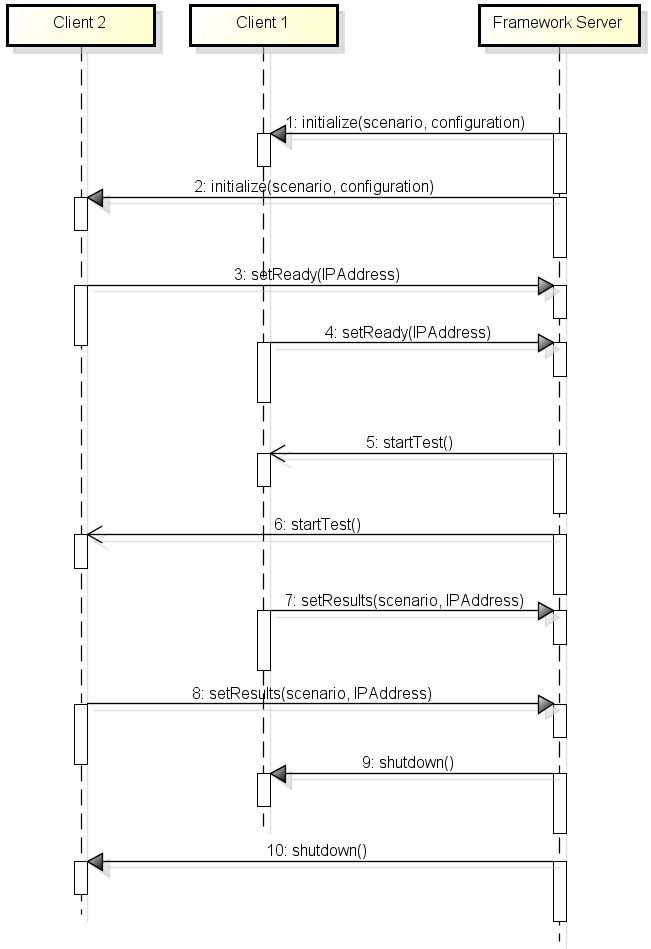
\includegraphics[scale=0.5]{image_testFramework/Server_Client_Communication.png}
\end{center}
\caption{Server Client Kommunikation}
\end{figure}

Die Umsetzung des Testframeworks wurde über das bewährte Client / Server Konzept realisiert, was zu einer schlanke Lösung auf Seiten des Clients führt. Der FrameworkClient und das ClientSystemUnderTest lassen sich dank die\-sem Konzept komplett vom Framework Server aus konfigurieren und steuern. Ein weiterer Vorteil dieses Designs liegt darin, dass sich neue Anforderungen jederzeit leicht umsetzen lassen.


\subsection{ClientController}
\label{sec:clientController}
 
Beim Start der client.jar Datei kann das Startup-Skript zwei Argumente mitgeben:
\begin{enumerate}
\item Pflicht Argument: Binding Namen
\item Optionales Argument: spezifischer RMI-Port
\end{enumerate}
Die Kommunikation zwischen dem Testframework Client und dem Testframework Server ist über das in Java bereits vorhandene RMI \cite{java_rmi} realisiert. Der Startvorgang eines Clients sieht wie folgt aus:
\begin{enumerate}
\item Es wird ein neues ClientController Objekt instanziiert. Der ClientController implementiert das Client Interface, welches mit Remote markiert ist.
\item Aus dem instanziierten ClientController Objekte wird ein Remoteobjekt generiert.
\item Der lokale Name Service wird auf dem spezifizierten Port gestartet, ist kein Port als Argument mitgegeben worden, wird der Defaultport 1099 verwendet.
\item Das ClientController Remoteobjekt lässt sich nun in dem Java Name Service unter dem angegeben Binding Name veröffentlichen. Der Server ist jetzt in der Lage ein ClientController Stub über die IP Adresse und den Binding Name zu lokalisieren.
\end{enumerate}

Über folgendes Client Interface wird der ClientController konfiguriert und gesteuert:
\begin{lstlisting}[language=java, breaklines=true] 	
public void initialize(Scenario scenario, Configuration configuration) throws RemoteException;
public void startTest() throws RemoteException;
public void shutdown() throws RemoteException;
\end{lstlisting}
Die Grundidee zu Beginn des Projekts war, dass alle Konfigurationswerte einzeln als Parameter an den ClientController übergeben werden. Es stellte sich je\-doch schon nach kurzer Zeit her\-aus, dass eine Kap\-se\-lung der be\-nötigen Para\-meter in einem seperaten Objekt eine wesentlich bessere Lösung darstellt. Dieses neue Datatransfer Objekt, beinhaltet sowohl alle nötigen Informationen für die Konfiguration des ClientSystemUnderTest als auch die des ClientControllers.

\subsubsection{Initialize des ClientControllers}
In der konkreten Im\-p\-le\-men\-ta\-ti\-on der Me\-tho\-de \texttt{initialize(Scenario sce\allowbreak na\allowbreak rio, Configuration configuration)} werden mehrer Auf\-gaben er\-le\-digt:
\begin{enumerate}
\item Aus dem Configuration Objekt wird die Server IP, der RMI Port und der Name unter dem der Framework Server registriert ist ausgelesen. Aus diesen Information wird eine neue RMI Verbindung zum Framework Server erzeugt.
\item Die Instanziierung des konkreten ClientSystemUnderTest übernimmt eine einzlne Klasse, welche als Factory implementiert ist. Der Factory wird nur der \verb+fully qualified name+, welcher im Configuration Objekt gespeichert ist, übergeben. Die Factory selbst instanziiert den ge\-wünschten Client\-System\-Under\-Test via Re\-flec\-ti\-on und re\-turniert das erzeugte Objekt.
\item Auf dem ClientSystemUnderTest Objekt wird nun ein neues Socket, welches zum ServerSystemUnderTest zeigt, gesetzt.
\item Ein neues Objekt vom Typ TestClient wird erzeugt und das aktuelle ClientSystemUnderTest Objekt wird im Konstruktor mitgegeben. Der TestClient ist die Schnittstelle zwischen dem ClientController und dem ClientSystemUnderTest.
\item Nun wird das Szenario, welches als Parameter übergeben wurde, auf dem TestClient Objekt gesetzt. 
\item Daraufhin wird auf dem Test\-Client Objekt die \verb+init()+ Methode auf\-ge\-rufen, in welcher sich der TestClient alle verfügbaren Account Objekte vom Server lädt.
\item Auf dem Testframework Server wird die Me\-tho\-de \verb+setReady()+ auf\-ge\-rufen, dieser Methoden\-aufruf teilt den Server mit, dass die Konfiguration des ClientControllers und des ClientSystemUnderTest erfolgreich war.
\item Im Anschluss wartet der der ClientController, bis der TestFramework Server den Testlauf startet.
\end{enumerate}

\subsubsection{Start eines Testlaufs}
\begin{figure}[H]
\begin{center}
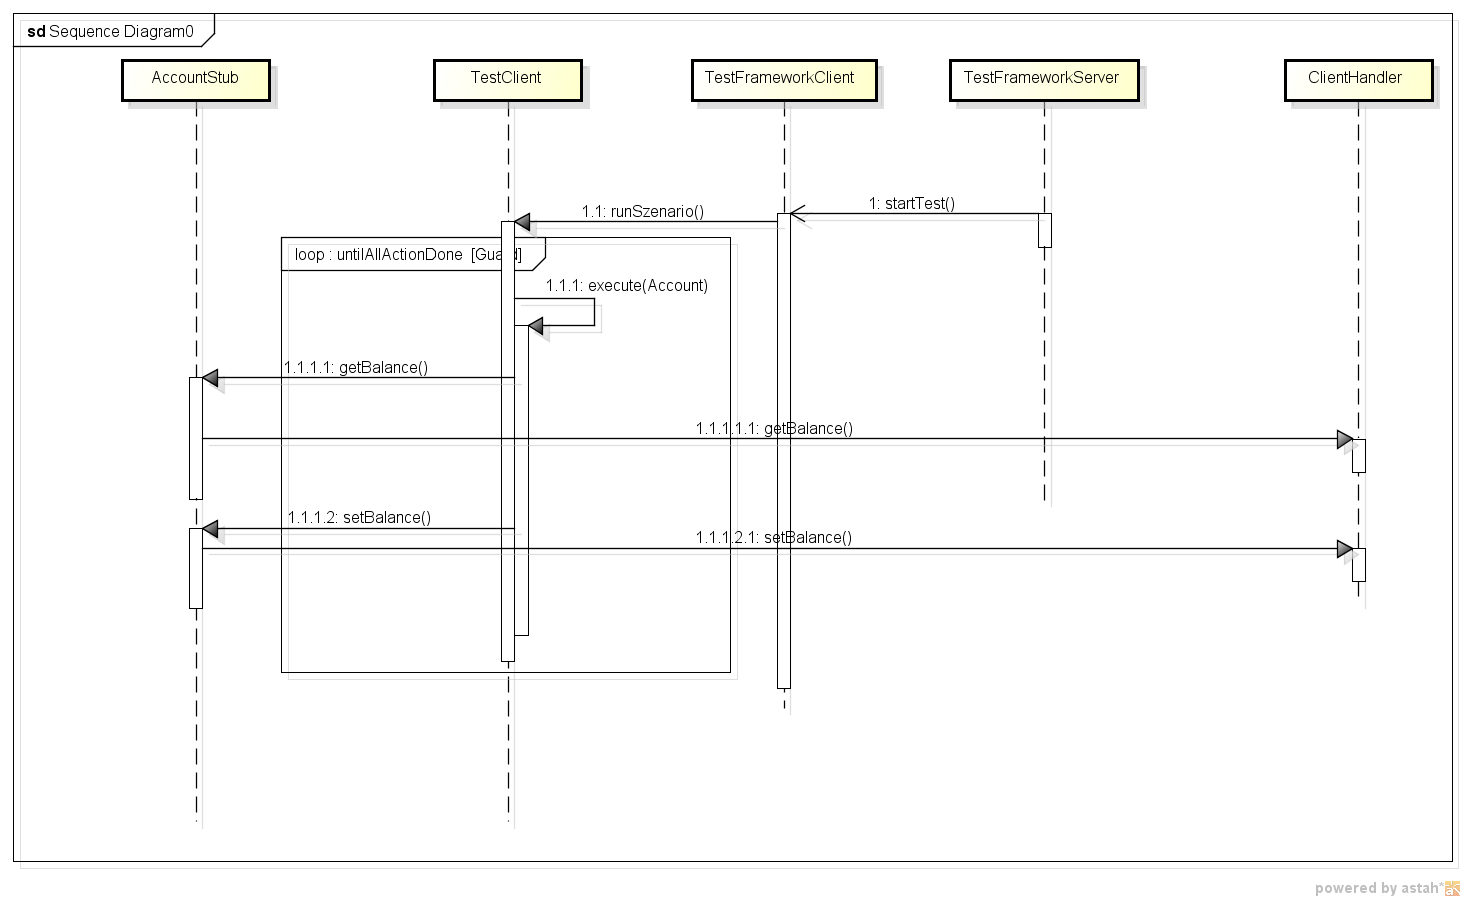
\includegraphics[scale=0.4]{image_testFramework/startTest.png}
\end{center}
\caption{Start eines Testlauf durch den Testframework Server}
\end{figure}
Das Sequenzdiagramm ist eine vereinfachte Darstellung des Testlaufs. Der Server startet den Testdurchlauf parallel auf allen ClientController über die Methode \verb+startTest()+. Diese ruft auf dem TestClient \verb+runScenario()+ auf, eine detailierte Erklärung was in dieser Methode passiert, ist im Kapitel "'Test Client" \ref{sec:testclient} zu finden. Sind alle Aktionen des gegeben Szenarios abgearbeitet, wird das gesamte Szenario mit den gesammelten Messresultaten über die Methode \verb+setResults(Scenario scenario, String IP)+ zurück an den Server geschickt.

\subsubsection{Herunterfahren des ClientController}
Die Methode \texttt{shutdown()} be\-endet den Test\-frame\-work\-Client und das Client\-System\-Under\-Test. Die \texttt{shut\allowbreak down()} Me\-tho\-de be\-steht aus mehreren Teil\-schrit\-ten:
\begin{enumerate}
\item Das ClientSystemUnderTest wird heruntergefahren.
\item Die Verbindung zwischen dem spezifizierten Binding Namen und dem damit verbundenen ClientController Remoteobjekt wird im Name Service von Java gelöscht.
\item Das ClientController Objekt wird von der RMI Run\-time entfernt, da\-durch sind keine RMI Aufrufe mehr möglich.
\item Der ClientController beendet sich selbst.
\end{enumerate}


Beim Testen der shutdown()-Funktionalität konnte festgestellt werden, dass bei der Umsetzung wie oben beschrieben, der Server immer eine Exception bekommt. Es stellte sich heraus, dass das sofortige Herunterfahren des ClientControllers nach dem Unbinding und dem Unexport des ClientController Objekts dem Server keine Zeit lässt, seine RMI Verbindung zum ClientController korrekt zu schliessen. Die Lösung des Problems lag in einer Pause zwischen dem Unexport und dem Beenden des ClientControllers. Die Dauer der Verzögerung von zwei Sekunden stellte sich als ausreichen heraus. Folgender Codeausschnitt zeigt die Lösung des Problems:
\begin{lstlisting}[language=java, breaklines=true]
private void shutdownClientController() throws RemoteException {
		try {
			Naming.unbind("rmi://localhost:" + ClientRmiPort + "/Client");
		} catch (MalformedURLException e1) {
			throw new RemoteException("Malformed URL has occurred in ClientController", e1);
		} catch (NotBoundException e1) {
			throw new RemoteException("Unbinding the ClientController failed", e1);
		}
		UnicastRemoteObject.unexportObject(this, true);
		closeClientController(2000);
	}

	private void closeClientController(final long delay) {
		new Thread() {
			@Override
			public void run() {
				logger.info("ClientController is shutting down");
				try {
					sleep(delay);
				} catch (InterruptedException e) {
				}
				System.exit(0);
			}
		}.start();
	}
}
\end{lstlisting}
Die Beendigung des ClientControllers wird in einem seperaten Thread ausgeführt, so\-dass der Main- Thread noch ge\-nü\-gend Zeit hat, alle of\-fe\-nen Ver\-bin\-dun\-gen ord\-nungs\-gemäss zu schliessen. Der Shutdown Thread beendet den ClientController nach der definierten Dauer mit \verb+System.exit()+.   

\subsection{Test Client}
\label{sec:testclient}
Die TestClient Klasse ist die Schnittstelle zwischen dem ClientController und dem ClientSystemUnderTest. Alle Clientvarianten die getestet werden sollen, müssen das Interface ClientSystemUnderTest implementieren, so lassen sich alle Varianten von ClientSystemUnderTest einheitlich mit einer TestClient Klasse testen. Desweiteren kann auf dem TestClient das Szenario gesetzt werden, welches der TestClient beim Aufruf von \verb+runScenario()+ durch den ClientController abarbeitet.

Das ClientSystemUnderTest Interface ist wie folgt definiert:
\begin{lstlisting}[language=java, breaklines=true] 	
public interface ClientSystemUnderTest {	
	public AccountService getAccountService();
	public void setServerSocketAdress(InetSocketAddress socketAdress);
	public void shutdown();
}	
\end{lstlisting}
\subsubsection{Ablauf}
\label{sec:ablauf}
\begin{enumerate}
\item Der ClientController setzt die Socket-Adresse des Server in das Client\-System\-Under\-Test. Die nötigen Imformationen sind im Configuration Objekt gespeichert.
\item Im Kon\-struk\-tor des Test\-Clients wird der Account\-Ser\-vice, des über\-ge\-be\-nen Client\-System\-Under\-Test über die Meth\-ode \texttt{get\allowbreak Account\allowbreak Ser\allowbreak vice()} ge\-la\-den. 
\item Während der Initialisierungsphase des ClientController ruft dieser ebenfalls die \verb+init()+ Methode des TestClients auf, in dieser Methode wird eine Liste aller verfügbaren Accounts Objekte aus dem AccountService in den TestClient geladen.
\item Startet der Server nun den Testlauf wird endlos durch die Liste der Accounts interiert bis alle Aktionen des gesetzten Szenarios abgearbeitet sind.
\item Bei einem Shutdown durch den Testframework Server ist der TestClient ebenfalls für die ord\-nungs\-ge\-mä\-sse Be\-en\-di\-gung des ClientSystemUnderTest zu\-stän\-dig.
\end{enumerate}

\subsubsection{Concurrency im TestClient}
\label{sec:concurrencyTestClient}
Während den ersten Testmessungen mit den Cache-System zeigte sich folgendes Problem: Der letzte TestClient, der sich beim Server als bereit meldet, benötigte für die ersten Aktionen im Durchschnitt etwa 40 Milisekunden länger als die restlichen Clients. Durch die Analyse des Codes konnte das Problem lokalisiert werden. Die folgenden Schritte zeigen die Ursache des Problems auf:
\begin{enumerate}
\item Der letzte Client meldet sich über die Methode \verb+setReady()+ beim Server als bereit. 
\item Beim Aufruf der \verb+setReady()+ Methode auf dem Server wird nun ge\-prüft, ob alle Clients bereit sind. Haben sich zuvor alle Clients als bereit für den Test\-lauf ge\-meldet, startet der Server auf jedem Client den Testlauf über die Methode \verb+startTest()+.
\item Zu diesem Zeitpunkt wartet der setReady Thread des letzten Clients immer noch auf die Rückkehr des Aufrufs.
\item Gleich\-zeit wird auf dem letzten Client die \verb+startTest()+ Methode auf\-gerufen. Da\-durch ent\-stehen beim letzten Client, der sich beim Server gemeldet hat, für kurze Zeit zwei Threads.
\item Ist die Methode \verb+setReady()+ erfolg\-reich durch\-laufen, kehrt der Auf\-ruf zum letzten Client zu\-rück. Da\-rauf\-hin be\-endet der Thread auf dem Client, welcher die \verb+setReady()+ Methode ge\-startet hat.
\item Gleichzeitig hat der \verb+startTest()+ Thread bereits begonnen mit dem abarbeiten des Szenarios. Da nun der Thread vom \verb+setReady()+ beendet wird, wird dem Szenario Thread die CPU-Ressource weggenommen. Dies führt nun zu einer Verlängerung der Ausführungsdauer der ersten Aktionen.
\end{enumerate}
Die Lösung dieses Problem lag in einer Wartephase vor dem eigentlichen Abarbeiten des Szenarios. Diese Pause wurde über \verb+Thread.sleep()+ um\-ge\-setzt und wird vor der eingent\-liche Messung ge\-macht. Da\-durch haben alle Client\-Controller Zeit, den \verb+setReady()+ Th\-read zu be\-enden, ohne den \verb+startTest()+ Th\-read zu be\-ein\-träch\-ti\-gen.



\section{Action}
\label{sec:action}
Ein Szenario beinhaltet eine Menge von Aktionen, welche auf ein Account Objekt ausgeführt werden können. Für eine einfache Erweiterbarkeit von neuen Aktionen, ist hierfür das Command-Pattern benutzt worden. Alle konkreten Implementierungen einer Aktion müssen von der abstrakte Klasse Action ableiten. Im Konstruktor dieser abstrakten Klasse wird ein neues Result Objekt instanziert. Im Kapitel "'Result" \ref{sec:result} wird dieser Typ genauer beschrieben. Dieses Objekt dient als Datenkontainer für alle Zeitmessungen die während dieser Aktion gesammelt werden sollen. Desweiteren deklariert Action drei abstrakte Methoden die von Subklassen implementiert werden müssen.
\begin{lstlisting}[language=java, breaklines=true] 	
public abstract ActionTyp getActionTyp();
public abstract int getMinimalNumberOfTimeRecords();
public abstract void execute(Account account);	
\end{lstlisting}

\begin{itemize}
\item Für eine detailierte Auswertung muss der Typ der Aktion zugänglich gemacht werden, dies ist über die Methode \verb+getActionTyp()+ möglich.
\item Eine Aktion be\-steht aus einer Ab\-folge von \texttt{get\allowbreak Balance()} und \texttt{set\allowbreak Balance()} Auf\-rufen. Je nach Aktion können mehrer Methodenaufrufe auf das Account Objekt nötig sein um die Aktion erfolgreich aus\-zu\-füh\-ren. Um im Reporting fest\-zu\-stellen, ob die Aktion beim ersten Versuch erfolg\-reich war, muss die minimale Anzahl von Time\-Records, in der Aktion ge\-speichert werden. Über die Me\-tho\-de \texttt{get\allowbreak Minimal\allowbreak Number\allowbreak Of\allowbreak Time\allowbreak Records()} lässt sich diese Zahl auslesen. So lassen sich Konflikte, die bei der Ausführung dieser Aktion auftreten, im Reporting feststellen.
\item Die Methode \verb+execute(Account account)+ beinhaltet die eigentlichen Methodenaufrufe, die auf dem Account-Objekt ausgeführt werden sollen. Das Account Objekt wird von TestClient an die Methode übergeben.
\end{itemize} 

\subsection{ActionTyp}
\label{sec:actionTyp}
Der ActionTyp wird zur Indentifizierung der Aktion benutzt und ist als Enum realisiert. Folgende Aktionstypen sind bereits vorhanden:
\begin{itemize}
\item \verb+ReadAction+
\item \verb+WriteAction+
\item \verb+IncrementAction+
\end{itemize}
Die Werte dieses Enums werden zur Erkennung des Aktiontyps genutzt und werden bei der Report Generierung verwendet, um die einzelnen Aktionen zu unterscheiden.

 
\subsection{Increment Action}
\label{sec:incrementAction}
Die Aktion \verb+IncrementAction+ ist die Kernaktion für alle Szenarien. Sie besteht aus drei Teilschritten:
\begin{itemize}
\item Über die Methode \verb+getBalance()+ den aktuellen Kontostand des Accounts abfragen und zwischenspeichern.
\item Den temporären Kontostand mit dem gegebenen Faktor multiplizieren.
\item Versuchen den neuen Wert via \verb+setBalance(balance)+ Methode zurück in das Konto, welches auf dem Server liegt, zu schreiben. 
\end{itemize}

\begin{lstlisting}[language=java, breaklines=true] 
@Override
public void execute(Account account) {
	boolean successful = false;
	double balance = 0;
	int numberOfTry = 0;
	while (!successful) {
		result.startTimeMeasurement(BasicAction.READ);
		balance = account.getBalance();
		result.stopTimeMeasurement();
		sleep(numberOfTry);
		try {
			result.startTimeMeasurement(BasicAction.WRITE);
			account.setBalance(balance * factor);
			result.stopTimeMeasurement();
			successful = true;
		} catch (RuntimeException e) {
			successful = false;
			result.stopTimeMeasurement(ActionResult.FAILED);
		}
		numberOfTry++;
	}
}
\end{lstlisting}
Im Laufe der Rea\-li\-sie\-rung stellte sich her\-aus das zwi\-schen dem \verb+getBalance()+ und dem \verb+setBalance()+-Auf\-ruf eine mi\-ni\-mal de\-fi\-nier\-ba\-re Zeit\-dauer ge\-wartet werden können muss. Diese Warteperiode ist nötig, damit sich leichter ein Konflikt erzeugen lässt und so gezeigt werden kann, dass der Fehler serverseitig zu keinem Lost-Updates führt. Tritt serverseitig ein Concurrency Fehler auf, wird eine RuntimeExeption zurück an den Client geworfen. Dieser Fehler veranlasst, dass die Aktion nochmals neu gestartet wird. Die Aktion wird solange wiederholt bis diese erfolgreich aus der While-Schleife kommt. Die Verzögerung zwischen dem Lesen und Schreiben, welche über die Methode \verb+sleep()+ realisiert ist, führt nur beim ersten Druchlauf der IncrementAction zu einer zeitlichen Verzögerung.

\subsection{WriteAction}
\label{sec:writeAction}
Die WriteAction wurde nur zu Beginn der Realisierung benutzt und schreibt via \verb+setBalance()+ einen gegeben Wert auf einen Account.

\subsection{ReadAction}
\label{sec:readAction}
Diese Aktion liest den aktuellen Kontostand eine Objekts und speichert diesen ab. Über \verb+getBalance()+ kann auf den Kontostand zugegriffen werden. Diese Aktion wurde für die Messungen benutzt.

\section{Result}
\label{sec:result}
Für die möglichst genaue Zeitmessung einer Aktion wird die von Java bereitgestellte Methode \verb+System.nanoTime()+ genutzt. Die Klasse "'Result" bietet eine \verb+startTimeMeasurement(BasicAction type)+ Methode, die ein neues TimeRecord Objekt erzeugt und die momentane Zeit in dieses TimeRecord Objekt schreibt. Die Information, ob es sich bei dieser Messung um eine lesende oder schreibende Methode handelt wird über denn BasicAction Typ an den TimeRecord weiter gegeben. Diese ist nötig, damit bei der Auswertung genau analysiert werden kann, für welchen Methodeaufruf (\verb+getBalance()+ / \verb+setBalance()+) dieser TimeRecord erzeugt wurde. Über die Methode \verb+stopTimeMeasurement(ActionResult result)+ lässt sich die Zeitmessung beenden und der aktuelle TimeRecord wird in einer Liste gespeichert. Das Argument, welches in der \verb+stopTimeMeasurment()+ Methode übergeben wird beinhaltet die Information über den Erfolg der Aktion. So lassen sich auch Aktionen erzeugen die aus mehreren \verb+getBalance()+ oder \verb+setBalance()+ Aufrufe bestehen. Dies ist zum Beispiel in der \texttt{Increment\allowbreak Action} der Fall.

\subsection{TimeRecord}
\label{sec:timeRecord}
Der TimeRecordtyp ist als reines Data Tranfer Object implementiert worden. Es beinhaltet die Start- und die Stopzeit von genau einem Methodenaufruf. Für eine genaue Auswertung einer Aktion sind noch weitere Daten nötig. Daher besitzt dieser Typ zwei weitere Felder. Der BasicActiontyp beinhaltet Informationen für welche Account Methode, also \verb+getBalance()+ oder \verb+setBalance()+, dieser Record gilt und in dem ActionResult kann die Information über den Erfolg der BasicAction gespeichert werden. Dadurch lassen sich zusammengesetzte Aktionen, welche aus \verb+getBalance()+ und \verb+setBalance()+ zusammengesetzt sind, einfach unterteilen. Ein weiterer Vorteil liegt in Mög\-lich\-keit ein Sze\-na\-rio bis die ein\-zel\-nen Me\-tho\-den Auf\-rufe einer Aktion zu analysieren. 

\subsection{BasicAction}
\label{sec:BasicAction}
Damit eine genaue Analyse der Aktionen ge\-macht werden kann, ist es nö\-tig, dass zwi\-schen \verb+getBalance()+ und \verb+setBalance()+ un\-ter\-schieden wer\-den kann. Eine Aktion kann aus einer Abfolge von Methoden\-auf\-rufen bestehen, daher muss bei jeder Zeitmessung angegeben werden können, ob es sich um eine "'setter" oder "'getter" Methode handelt, diese Information lässt sich daher ebenfalls im TimeRecord speichern.

\subsection{ActionResult}
\label{sec:ActionResult}
Den Erfolg eines \verb+getBalance()+ oder \verb+setBalance()+ Aufrufs lässt sich ebenfalls im TimeRecord speichern. Dies Hilft die Fehlerrate eines Methodenaufrufe zu ermitteln, daher ist es nötig, dass beim Stoppen einer Messung der Erfolgstatus gespeichert wird.




